\chapter{Working with bipolar-valued digraphs}
\label{sec:2}

\abstract*{To be written.}

\abstract{To be written.}

\section{Random bipolar-valued digraphs}

We are starting this tutorial with generating a uniformly random $[-1.0; +1.0]$-valued digraph of order 7, denoted $rdg$ and modelling, for instance, a binary relation $S(x,y)$ defined on the set of nodes of $rdg$. For this purpose, the \Digraph3 resources provide a {\tt randomDigraphs} module providing a specific {\tt RandomValuationDigraph} constructor.

\begin{lstlisting}[caption={Random bipolar-valued digraph instance},label=list:2.1]
   >>> from randomDigraphs import RandomValuationDigraph
   >>> rdg = RandomValuationDigraph(order=7)
   >>> rdg.save('tutRandValDigraph')
   >>> from digraphs import Digraph
   >>> rdg = Digraph('tutRandValDigraph')
   >>> rdg
    *------- Digraph instance description ------*
    Instance class      : Digraph
    Instance name       : tutRandValDigraph
    Digraph Order       : 7
    Digraph Size        : 22
    Valuation domain    : [-1.00;1.00]
    Determinateness (%) : 75.24
    Attributes          : ['name','actions','order',
                           'valuationdomain','relation',
                           'gamma','notGamma']
\end{lstlisting}   

With the {\tt Digraph.save()} method (see Listing \ref{list:2.1} Line 3) we may keep a backup version for future use of $rdg$ which will be stored in a file called {\tt tutRandValDigraph.py} in the current working directory. The genuine {\tt Digraph} class constructor may restore the $rdg$ object from the stored file (Line 4-5). We may easily inspect the content of $rdg$ (Line 5). The digraph size 22 indicates the number of positively valued arcs. The valuation domain is uniformly distributed in the interval $[-1.0; 1.0]$ and the mean absolute arc valuation is $(0.7524 \times 2)\, -\, 1.0 \;=\; 0.5048$ (Line 12) .

All objects of {\tt Digraph} type contain at least the list of attributes shown here: a \texttt{name} (string), a dictionary of \texttt{actions} (digraph nodes), an \texttt{order} (integer) attribute containing the number of actions, a \texttt{valuationdomain} dictionary, a double dictionary \texttt{relation} representing the adjency table of the digraph relation, a \texttt{gamma} and a {\tt notGamma} dictionary containing the direct neighbourhood of each action.

As mentioned in the previous Chapter, the {\tt Digraph} class provides some generic {\tt show} methods for exploring a given {\tt Digraph} object, like the {\tt showShort()}, {\tt showAll()}, {\tt showRelationTable()} and the {\tt showNeighborhoods()} methods.

\begin{lstlisting}[caption={Example of random valuation digraph},label=list:2.2]
   >>> rdg.showAll()
    *----- show detail -------------*
     Digraph          : tutRandValDigraph
    *---- Actions ----*
     ['1', '2', '3', '4', '5', '6', '7']
    *---- Characteristic valuation domain ----*
     {'med': Decimal('0.0'), 'hasIntegerValuation': False, 
      'min': Decimal('-1.0'), 'max': Decimal('1.0')}
    * ---- Relation Table -----
    r(xSy) |  '1'    '2'   '3'  '4'   '5'    '6'  '7'	  
    -------|-------------------------------------------
    '1'    |  0.00 -0.48  0.70  0.86  0.30  0.38  0.44	 
    '2'    | -0.22  0.00 -0.38  0.50  0.80 -0.54  0.02	 
    '3'    | -0.42  0.08  0.00  0.70 -0.56  0.84 -1.00	 
    '4'    |  0.44 -0.40 -0.62  0.00  0.04  0.66  0.76	 
    '5'    |  0.32 -0.48 -0.46  0.64  0.00 -0.22 -0.52	 
    '6'    | -0.84  0.00 -0.40 -0.96 -0.18  0.00 -0.22	 
    '7'    |  0.88  0.72  0.82  0.52 -0.84  0.04  0.00
    *--- Connected Components ---*
     1: ['1', '2', '3', '4', '5', '6', '7']
    Neighborhoods:
     Gamma:
     '1': in => {'5', '7', '4'}, out => {'5', '7', '6', '3', '4'}
     '2': in => {'7', '3'}, out => {'5', '7', '4'}
     '3': in => {'7', '1'}, out => {'6', '2', '4'}
     '4': in => {'5', '7', '1', '2', '3'}, out => {'5', '7', '1', '6'}
     '5': in => {'1', '2', '4'}, out => {'1', '4'}
     '6': in => {'7', '1', '3', '4'}, out => set()
     '7': in => {'1', '2', '4'}, out => {'1', '2', '3', '4', '6'}
     Not Gamma:
     '1': in => {'6', '2', '3'}, out => {'2'}
     '2': in => {'5', '1', '4'}, out => {'1', '6', '3'}
     '3': in => {'5', '6', '2', '4'}, out => {'5', '7', '1'}
     '4': in => {'6'}, out => {'2', '3'}
     '5': in => {'7', '6', '3'}, out => {'7', '6', '2', '3'}
     '6': in => {'5', '2'}, out => {'5', '7', '1', '3', '4'}
     '7': in => {'5', '6', '3'}, out => {'5'}
\end{lstlisting}   

\begin{svgraybox}
 Mind that most Digraph class methods will ignore the \emph{reflexive} links by considering that they are \emph{indeterminate}, i.e. the characteristic value $r(x\,S\,x)$ for all action $x$ is set to the \emph{median}, i.e. \emph{indeterminate} value $0.0$ in this case (see Listing \ref{list:2.2} Lines 12-18 and [BIS-2004a]).
 \end{svgraybox}

\section{Graphviz drawings}
\label{sec:2.2}

We may have an even better insight into the \texttt{Digraph} object $rdg$ by looking at a \href{https://graphviz.org/}{graphviz} drawing [Footnote 1].

\begin{lstlisting}
>>> rdg.exportGraphViz('tutRandValDigraph')
 *---- exporting a dot file for GraphViz tools ---------*
  Exporting to tutRandValDigraph.dot
  dot -Grankdir=BT -Tpng tutRandValDigraph.dot -o tutRandValDigraph.png
\end{lstlisting}

\begin{figure}[h]
\sidecaption
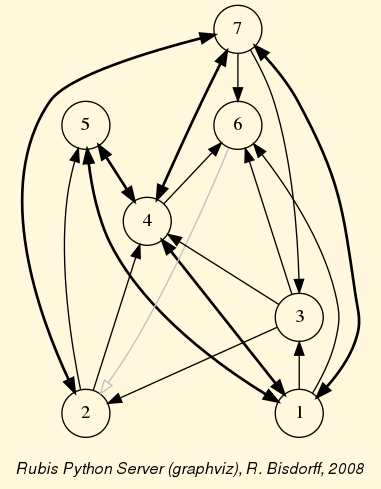
\includegraphics[width=6cm]{Figures/tutRandValDigraph.png}
\caption{The tutorial random valuation digraph. Double links are drawn in bold black with an arrowhead at each end, whereas single asymmetric links are drawn in black with an arrowhead showing the direction of the link. Notice the undetermined relational situation ($r(6\,S\,2) = 0.00$) observed between nodes '6' and '2'. The corresponding link is marked in gray with an open arrowhead in the drawing.}
\label{fig:2.1}       % Give a unique label
\end{figure}
  
\section{Asymmetric and symmetric parts}
\label{sec:2.3}

We may now extract both the \emph{}\emph{symmetric} as well as the asymmetric part of digraph $dg$ with the help of two corresponding constructors (see Listing \ref{list:2.3}).

\begin{lstlisting}[caption={Computing asymmetric and symmetric Parts},label=list:2.3]
>>> from digraphs import AsymmetricPartialDigraph,\
...                      SymmetricPartialDigraph
   
>>> asymDg = AsymmetricPartialDigraph(rdg)
>>> asymDg.exportGraphViz()
>>> symDg = SymmetricPartialDigraph(rdg)
>>> symDg.exportGraphViz()
\end{lstlisting}

\begin{figure}[h]
%\sidecaption
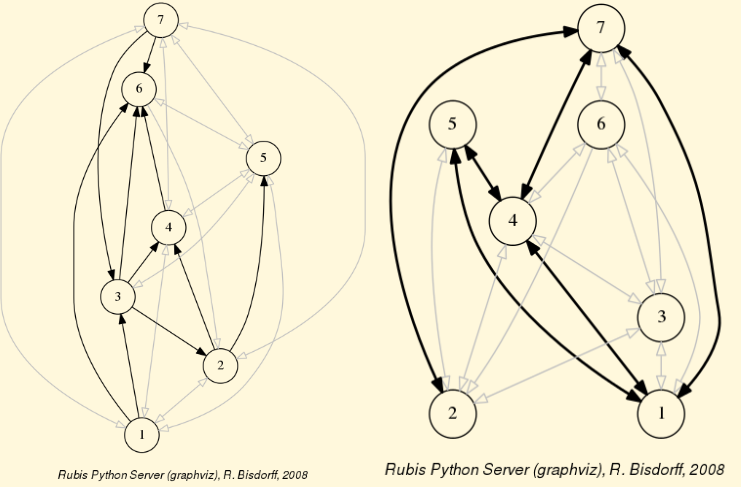
\includegraphics[width=11cm]{Figures/asymSymParts.png}
\caption{Asymmetric and symmetric part of the tutorial random valuation digraph.}
\label{fig:2.2}       % Give a unique label
\end{figure}
  
\begin{svgraybox}The constructor of the partial objects $asymDg$ and $symDg$ puts to the indeterminate characteristic value all not-asymmetric, respectively not-symmetric links between nodes (see Fig. \ref{fig:2.2}).
 \end{svgraybox}

Here below, for illustration the source code of the {\tt relation} constructor of the {\tt AsymmetricPartialDigraph} class.

\begin{lstlisting}[label=list:2.4,basicstyle=\footnotesize]
    def _constructRelation(self):
	actions = self.actions
	Min = self.valuationdomain['min']
	Max = self.valuationdomain['max']
	Med = self.valuationdomain['med']
	relationIn = self.relation
	relationOut = {}
	for a in actions:
	    relationOut[a] = {}
	    for b in actions:
		if a != b:
		    if relationIn[a][b] >= Med and relationIn[b][a] <= Med:
			relationOut[a][b] = relationIn[a][b]
		    elif relationIn[a][b] <= Med and relationIn[b][a] >= Med:
			relationOut[a][b] = relationIn[a][b]
		    else:
			relationOut[a][b] = Med
		else:
		    relationOut[a][b] = Med
	return relationOut
\end{lstlisting}

\section{Border and inner parts}
\label{sec:2.4}

We may also extract the border -the part of a digraph induced by the union of its initial and terminal prekernels (see Kernel Chapter)-  as well as, the inner part -the complement of the border- with the help of two corresponding class constructors: \texttt{GraphBorder} and \texttt{GraphInner} (see Fig. \ref{fig:2.3}).

Let us illustrate these parts on a linear ordering obtained from the tutorial random valuation digraph $rdg$  with the \NetFlows ranking rule  (see Section \ref{sec:8.3}).  

\begin{lstlisting}[caption={Border and inner part of a linear order},label=list:2.5]
>>> from digraphs import GraphBorder, GraphInner
>>> from linearOrders import NetFlowsOrder
>>> nf = NetFlowsOrder(rdg)
>>> nf.netFlowsOrder
   ['6', '4', '5', '3', '2', '1', '7']
>>> bnf = GraphBorder(nf)
>>> bnf.exportGraphViz(worstChoice=['6'],bestChoice=['7'])
>>> inf = GraphInner(nf)
>>> inf.exportGraphViz(worstChoice=['6'],bestChoice=['7'])
\end{lstlisting}

\begin{figure}[h]
%\sidecaption
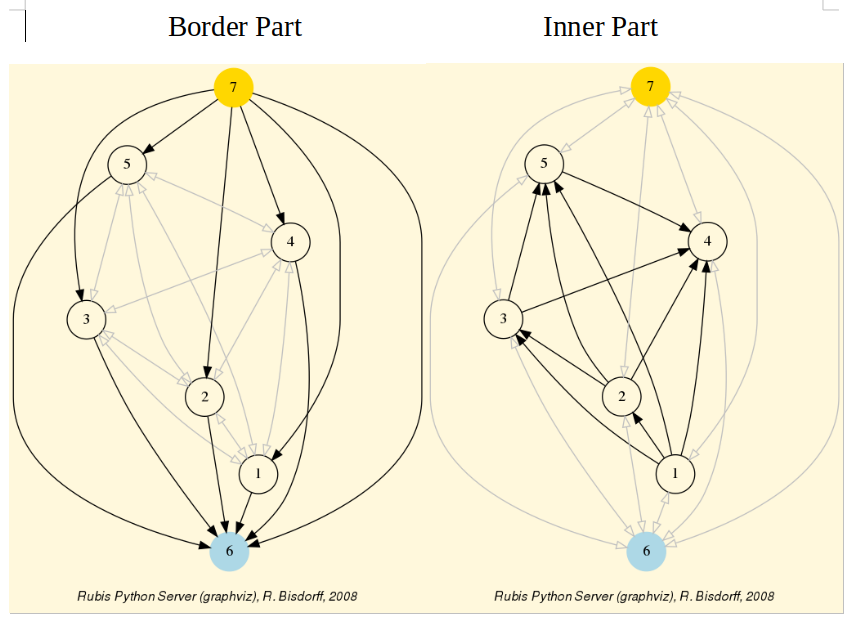
\includegraphics[width=11cm]{Figures/graphBorderAndInner1.png}
\caption{\emph{Border} and \emph{inner} part of a linear order oriented by \emph{terminal} and \emph{initial} kernels.}
\label{fig:2.3}       % Give a unique label
\end{figure}
   
We may orient the \texttt{graphviz} drawings in Fig. \ref{fig:2.3}  with the terminal node 6 (\texttt{worstChoice} parameter) and initial node 7 (\texttt{bestChoice} parameter) (see Listing \ref{list:2.5} Lines 7 and 9).

\begin{svgraybox}The constructor of the partial digraphs $bnf$ and $inf$  (see Lines 3 and 6) puts to the \emph{indeterminate} characteristic value all links not in the \emph{border}, respectively \emph{not} in the \emph{inner} part (see Fig. \ref{fig:2.3}).\end{svgraybox}

Being much {\em denser\/} than a linear order, the actual inner part of our tutorial random valuation digraph $dg$ is reduced to a single arc between nodes 3 and 4 (see Fig. \ref{fig:2.4}).
   
\begin{figure}[h]
%\sidecaption
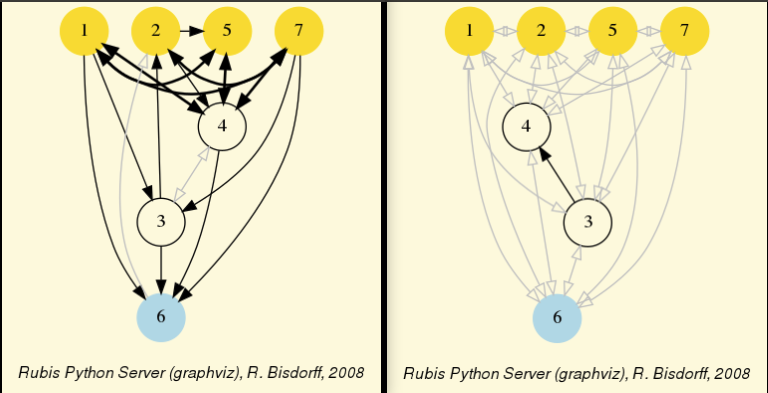
\includegraphics[width=11cm]{Figures/graphBorderAndInner.png}
\caption{Border and inner part of the tutorial random valuation digraph $rdg$.}
\label{fig:2.4}       % Give a unique label
\end{figure}
  
Indeed, a complete digraph on the limit has no inner part (privacy!) at all, whereas empty and indeterminate digraphs admit both, an empty border and an empty inner part.

\section{Fusion by epistemic disjunction}
\label{sec:2.5}

We may recover object $rdg$ from both partial objects $asymDg$ and $symDg$, or as well from the border $bg$ and the inner part $ig$, with a \textbf{bipolar fusion} constructor, also called \textbf{epistemic disjunction}, available via the \texttt{FusionDigraph} class. 

\begin{lstlisting}[caption={Epistemic fusion of partial diagraphs},label=list:2.6]
   >>> from digraphs import FusionDigraph
   >>> fusDg = FusionDigraph(asymDg,symDg,operator='o-max')
   >>> # fusDg = FusionDigraph(bg,ig,operator='o-max')
   >>> fusDg.showRelationTable()
    * ---- Relation Table -----
    r(xSy) |  '1'    '2'   '3'  '4'   '5'    '6'  '7'	  
    -------|------------------------------------------
    '1'    |  0.00 -0.48  0.70  0.86  0.30  0.38  0.44	 
    '2'    | -0.22  0.00 -0.38  0.50  0.80 -0.54  0.02	 
    '3'    | -0.42  0.08  0.00  0.70 -0.56  0.84 -1.00	 
    '4'    |  0.44 -0.40 -0.62  0.00  0.04  0.66  0.76	 
    '5'    |  0.32 -0.48 -0.46  0.64  0.00 -0.22 -0.52	 
    '6'    | -0.84  0.00 -0.40 -0.96 -0.18  0.00 -0.22	 
    '7'    |  0.88  0.72  0.82  0.52 -0.84  0.04  0.00
\end{lstlisting}
The epistemic fusion operator \texttt{o-max} (see Listing \ref{list:2.6} Line 2) works as follows.

Let $r$ and $r'$ characterise two bipolar-valued epistemic situations.
\begin{itemize}
\item $o-max(r, r' ) = \max(r, r' )$ when both $r$ and $r'$ are more or less valid or indeterminate;
\item $o-max(r, r' ) = \min(r, r' )$ when both $r$ and $r'$ are more or less invalid or indeterminate;
\item $o-max(r, r' ) = 0.0$, i.e. indeterminate otherwise.
\end{itemize}

\section{Dual, converse and codual digraphs}
\label{sec:2.6}

We may as readily compute the \textbf{dual} (negated relation Footnote[14]), the \textbf{converse} (transposed relation) and the \textbf{codual} (transposed and negated relation) of the digraph instance $rdg$. 

\begin{lstlisting}[caption={Computing dual, converse and codual},label=list:2.7]
>>> from digraphs import DualDigraph, ConverseDigraph, CoDualDigraph
>>> ddg = DualDigraph(rdg)
>>> ddg.showRelationTable()
    -r(xSy) |  '1'    '2'   '3'  '4'   '5'    '6'  '7'	  
    --------|------------------------------------------
    '1 '    |  0.00  0.48 -0.70 -0.86 -0.30 -0.38 -0.44	 
    '2'     |  0.22  0.00  0.38 -0.50  0.80  0.54 -0.02	 
    '3'     |  0.42  0.08  0.00 -0.70  0.56 -0.84  1.00	 
    '4'     | -0.44  0.40  0.62  0.00 -0.04 -0.66 -0.76	 
    '5'     | -0.32  0.48  0.46 -0.64  0.00  0.22  0.52	 
    '6'     |  0.84  0.00  0.40  0.96  0.18  0.00  0.22	 
    '7'     |  0.88 -0.72 -0.82 -0.52  0.84 -0.04  0.00

>>> cdg = ConverseDigraph(rdg)
>>> cdg.showRelationTable()
    * ---- Relation Table -----
     r(ySx) |  '1'    '2'   '3'   '4'   '5'   '6'   '7'	  
    --------|------------------------------------------
    '1'     |  0.00 -0.22 -0.42  0.44  0.32 -0.84  0.88	 
    '2'     | -0.48  0.00  0.08 -0.40 -0.48  0.00  0.72	 
    '3'     |  0.70 -0.38  0.00 -0.62 -0.46 -0.40  0.82	 
    '4'     |  0.86  0.50  0.70  0.00  0.64 -0.96  0.52	 
    '5'     |  0.30  0.80 -0.56  0.04  0.00 -0.18 -0.84	 
    '6'     |  0.38 -0.54  0.84  0.66 -0.22  0.00  0.04	 
    '7'     |  0.44  0.02 -1.00  0.76 -0.52 -0.22  0.00	 

>>> cddg = CoDualDigraph(rdg)
>>> cddg.showRelationTable()
    * ---- Relation Table -----
    -r(ySx) |  '1'    '2'   '3'   '4'   '5'   '6'   '7'	    
    --------|------------------------------------------
    '1'     |  0.00  0.22  0.42 -0.44 -0.32  0.84 -0.88	 
    '2'     |  0.48  0.00 -0.08  0.40  0.48  0.00 -0.72	 
    '3'     | -0.70  0.38  0.00  0.62  0.46  0.40 -0.82	 
    '4'     | -0.86 -0.50 -0.70  0.00 -0.64  0.96 -0.52	 
    '5'     | -0.30 -0.80  0.56 -0.04  0.00  0.18  0.84	 
    '6'     | -0.38  0.54 -0.84 -0.66  0.22  0.00 -0.04	 
    '7'     | -0.44 -0.02  1.00 -0.76  0.52  0.22  0.00	 
\end{lstlisting}
  
Computing the dual, respectively the converse of a dograph, may also be done with prefixing the \texttt{\_\_neg\_\_} ($-$) or the \texttt{\_\_invert\_\_} ($\sim$) operator. The codual of a \texttt{Digraph} object may, hence, as well be computed with a \textbf{composition} (in either order) of both operations.

\begin{lstlisting}[caption={Computing the dual, the converse and the codual of a digraph},label=list:2.8]
>>> ddg = -rdg   # dual of rdg
>>> cdg = ~rdg   # converse of rdg
>>> cddg = ~(-rdg) # = -(~(rdg) codual of rdg
>>> (-(~rdg)).showRelationTable()
  * ---- Relation Table -----
   -r(ySx) |  '1'    '2'   '3'   '4'   '5'   '6'   '7'	    
   --------|------------------------------------------
   '1'     |  0.00  0.22  0.42 -0.44 -0.32  0.84 -0.88	 
   '2'     |  0.48  0.00 -0.08  0.40  0.48  0.00 -0.72	 
   '3'     | -0.70  0.38  0.00  0.62  0.46  0.40 -0.82	 
   '4'     | -0.86 -0.50 -0.70  0.00 -0.64  0.96 -0.52	 
   '5'     | -0.30 -0.80  0.56 -0.04  0.00  0.18  0.84	 
   '6'     | -0.38  0.54 -0.84 -0.66  0.22  0.00 -0.04	 
   '7'     | -0.44 -0.02  1.00 -0.76  0.52  0.22  0.00	 
\end{lstlisting}
  
\section{Symmetric and transitive closures}
\label{sec:2.7}

Symmetric and transitive closures, by default in-site constructors, are also available (see Fig. \ref{fig:2.5}). Note that it is a good idea, before going ahead with these in-site operations, who irreversibly modify the original $rdg$ object, to previously make a backup version of $rdg$. The simplest storage method, always provided by the generic \texttt{Digraph.save()}, writes out in a named file the python content of the Digraph object in string representation (see Section \ref{sec:1.x}).

\begin{lstlisting}[caption={Symmeric and transitive closures},label=list:2.9]
>>> rdg.save('tutRandValDigraph')
>>> rdg.closeSymmetric(InSite=True)
>>> rdg.closeTransitive(InSite=True)
>>> rdg.exportGraphViz('strongComponents')
\end{lstlisting}

\begin{figure}[h]
\sidecaption
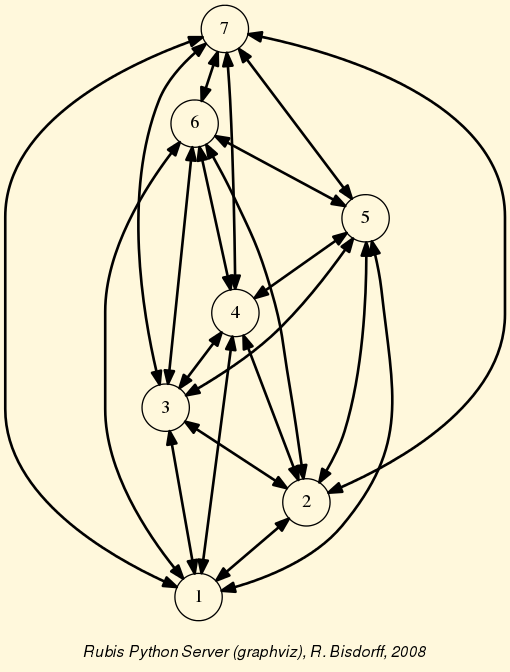
\includegraphics[width=6cm]{Figures/strongComponents.png}
\caption{Symmetric and transitive closure of the tutorial random valuation digraph $rdg$.}
\label{fig:2.5}       % Give a unique label
\end{figure}
 
The \texttt{closeSymmetric()} method (see Listing \ref{list:2.9}  Line 2), of complexity $O(n^2)$ where $n$ denotes the digraph's order, changes, on the one hand, all single pairwise links it may detect into double links by operating a disjunction of the pairwise relations. On the other hand, the \texttt{closeTransitive()} method (see Line 3), implements the \emph{Roy-Warshall} transitive closure algorithm of complexity $O(n^3)$. (Fotnote [17])

\begin{svgraybox}The same closeTransitive() method with a \texttt{Reverse = True} flag may be readily used for eliminating all transitive arcs from a transitive digraph instance. We make usage of this feature when drawing Hasse diagrams of \texttt{TransitiveDigraph} objects.\end{svgraybox}

\section{Strong components}
\label{sec:2.8}

As the original digraph $rdg$ was connected (see above the result of the showShort() command), both the symmetric and the transitive closures operated together, will necessarily produce a single strong component, i.e. a \textbf{complete} digraph. We may sometimes wish to collapse all strong components in a given digraph and construct the so \emph{collapsed} digraph. Using the \texttt{StrongComponentsCollapsedDigraph} constructor here will render a single hyper-node gathering all the original nodes (see Line 7 below).

\begin{lstlisting}[caption={Computing strong components},label=list:2.10]
>>> from digraphs import StrongComponentsCollapsedDigraph
>>> sc = StrongComponentsCollapsedDigraph(dg)
>>> sc.showAll()
  *----- show detail -----*
   Digraph          : tutRandValDigraph_Scc

  *---- Actions ----*
    ['_7_1_2_6_5_3_4_']

  * ---- Relation Table -----
      S     |  'Scc_1'	  
     -------|---------

  'Scc_1' |  0.00	 
   short 	 content
   Scc_1 	 _7_1_2_6_5_3_4_

   Neighborhoods:
   Gamma     :
   'frozenset({'7','1','2','6','5','3','4'})':
                     in => set(), out => set()
   Not Gamma :
   'frozenset({'7','1','2','6','5','3','4'})':
                     in => set(), out => set()
\end{lstlisting}
  
\section{CSV storage}
\label{sec:2.9}

Sometimes it is required to exchange the graph valuation data in CSV format with a statistical package like \href{https://www.r-project.org/}{R}. For this purpose it is possible to export the digraph data into a CSV file. The valuation domain is hereby normalized by default to the range $[-1.0,1.0]$ and the diagonal is put by default to the minimal value $-1.0$.

\begin{lstlisting}
>>> rdg = Digraph('tutRandValDigraph')
>>> rdg.saveCSV('tutRandValDigraph')
  # content of file tutRandValDigraph.csv
  "d","1","2","3","4","5","6","7"
  "1",-1.0,0.48,-0.7,-0.86,-0.3,-0.38,-0.44
  "2",0.22,-1.0,0.38,-0.5,-0.8,0.54,-0.02
  "3",0.42,-0.08,-1.0,-0.7,0.56,-0.84,1.0
  "4",-0.44,0.4,0.62,-1.0,-0.04,-0.66,-0.76
  "5",-0.32,0.48,0.46,-0.64,-1.0,0.22,0.52
  "6",0.84,0.0,0.4,0.96,0.18,-1.0,0.22
  "7",-0.88,-0.72,-0.82,-0.52,0.84,-0.04,-1.0
\end{lstlisting}
  
It is possible to reload a \texttt{Digraph} instance from its previously saved CSV file content.

\begin{lstlisting} 
>>> from digraphs import CSVDigraph   
>>> rdgcsv = CSVDigraph('tutRandValDigraph')
>>> rdgcsv.showRelationTable(ReflexiveTerms=False)
    * ---- Relation Table -----
    r(xSy) |   '1'   '2'   '3'   '4'   '5'   '6'   '7'	  
    -------|------------------------------------------------------------
    '1'    |   -   -0.48  0.70  0.86  0.30  0.38  0.44	 
    '2'    | -0.22   -   -0.38  0.50  0.80 -0.54  0.02	 
    '3'    | -0.42  0.08   -    0.70 -0.56  0.84 -1.00	 
    '4'    |  0.44 -0.40 -0.62   -    0.04  0.66  0.76	 
    '5'    |  0.32 -0.48 -0.46  0.64   -   -0.22 -0.52	 
    '6'    | -0.84  0.00 -0.40 -0.96 -0.18   -   -0.22	 
    '7'    |  0.88  0.72  0.82  0.52 -0.84  0.04   -
\end{lstlisting}
  
It is as well possible to show a colored version of the valued relation table in a system browser window tab (see Fig. \ref{fig:2.5}).

\begin{lstlisting}
>>> rdgcsv.showHTMLRelationTable(tableTitle="Tutorial random digraph")
\end{lstlisting}
 
\begin{figure}[h]
\sidecaption
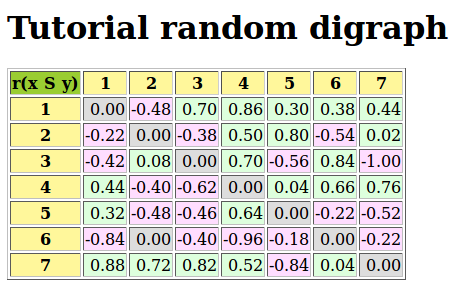
\includegraphics[width=5cm]{Figures/htmlTutorialDigraph.png}
\caption{The valued relation table shown in a browser window. Positive arcs are shown in *green* and negative arcs in *red*. Indeterminate -zero-valued- links, like the reflexive diagonal ones or the link between node *6* and node *2*, are shown in *gray*.}
\label{fig:2.6}       % Give a unique label
\end{figure}
 
\section{Complete, empty and indeterminate digraphs}
\label{sec:2.10}

Let us finally mention some special universal classes of digraphs that are readily available in the :py:mod:`digraphs` module, like the \texttt{CompleteDigraph}, the \texttt{EmptyDigraph} and the \texttt{IndeterminateDigraph} classes, which put all characteristic values respectively to the maximum, the minimum or the median indeterminate characteristic value.

\begin{lstlisting}[caption={Complete, empty and indeterminate digraphs},label=list:2.11]
>>> from digraphs import CompleteDigraph,EmptyDigraph,\
...   			 IndeterminateDigraph
   
>>> e = EmptyDigraph(order=5)
>>> e.showRelationTable()
    * ---- Relation Table -----
      S   |    '1'    '2'    '3'    '4'	   '5'	  
    ---- -|-----------------------------------
    '1'   |  -1.00  -1.00  -1.00  -1.00	 -1.00	 
    '2'   |  -1.00  -1.00  -1.00  -1.00	 -1.00	 
    '3'   |  -1.00  -1.00  -1.00  -1.00	 -1.00	 
    '4'   |  -1.00  -1.00  -1.00  -1.00	 -1.00	 
    '5'   |  -1.00  -1.00  -1.00  -1.00	 -1.00

>>> e.showNeighborhoods() 
    Neighborhoods:
      Gamma     :
    '1': in => set(), out => set()
    '2': in => set(), out => set()
    '5': in => set(), out => set()
    '3': in => set(), out => set()
    '4': in => set(), out => set()
      Not Gamma :
    '1': in => {'2', '4', '5', '3'}, out => {'2', '4', '5', '3'}
    '2': in => {'1', '4', '5', '3'}, out => {'1', '4', '5', '3'}
    '5': in => {'1', '2', '4', '3'}, out => {'1', '2', '4', '3'}
    '3': in => {'1', '2', '4', '5'}, out => {'1', '2', '4', '5'}
    '4': in => {'1', '2', '5', '3'}, out => {'1', '2', '5', '3'}

>>> i = IndeterminateDigraph()
    * ---- Relation Table -----
      S   |   '1'   '2'	  '3'	'4'   '5'	  
    ------|------------------------------
    '1'   |  0.00  0.00	 0.00  0.00  0.00	 
    '2'   |  0.00  0.00	 0.00  0.00  0.00	 
    '3'   |  0.00  0.00	 0.00  0.00  0.00	 
    '4'   |  0.00  0.00	 0.00  0.00  0.00	 
    '5'   |  0.00  0.00	 0.00  0.00  0.00	 

>>> i.showNeighborhoods()
    Neighborhoods:
      Gamma     :
    '1': in => set(), out => set()
    '2': in => set(), out => set()
    '5': in => set(), out => set()
    '3': in => set(), out => set()
    '4': in => set(), out => set()
      Not Gamma :
    '1': in => set(), out => set()
    '2': in => set(), out => set()
    '5': in => set(), out => set()
    '3': in => set(), out => set()
    '4': in => set(), out => set()
\end{lstlisting}

\begin{svgraybox}Mind the subtle difference between the neighborhoods of an \textbf{empty} and the neighborhoods of an \textbf{indeterminate} digraph instance. In the first kind, the neighborhoods are known to be completely \emph{empty}  (see Listing \ref{list:2.11} Lines 22-27) whereas, in the latter, \emph{nothing is known} about the actual neighborhoods of the nodes  (see Lines 45-50). These two cases illustrate why in the case of \textbf{bipolar-valued} digraphs, we may need both a \texttt{gamma} \textbf{and} a \texttt{notGamma} attribute.
  \end{svgraybox}
